\documentclass[a4paper,11pt, notitlepage]{article}

\usepackage[utf8]{inputenc}
\usepackage[T1]{fontenc}

\usepackage[top=2.5cm, bottom=3cm, left=3cm, right=3cm, headsep=14pt]{geometry}
\usepackage{graphicx}
\graphicspath{{images/}}
\usepackage[export]{adjustbox}

\usepackage{datetime}
\usepackage{float}
\usepackage{a4wide}
\usepackage[super]{nth}
\usepackage{mathtools}
\usepackage{hyperref}
\usepackage{fancyvrb}
\usepackage{booktabs}
\usepackage{multirow}
\usepackage{caption}

\usepackage{natbib}
\bibliographystyle{unsrt}


\setlength{\parskip}{0.5em}

\begin{document}

\title{
\vspace{-3cm}
Report 5 - Gaussian Blur}
\author{Nguyen Nhu Khoa - M.ICT.06.003}
\maketitle

\pagestyle{plain}
\setcounter{page}{1}

\vspace{-1cm}
\newdate{date}{31}{10}{2017}
\noindent
\section{GPU Gaussian Blur Implementation}
\begin{flushleft}
\small
\begin{BVerbatim}
__global__ void gaussianConvolution(unsigned char *input, 
			unsigned char *output, int imageWidth, 
				int imageHeight, int pixelCount){
    int gKernel[7][7] = {{0, 0, 1, 2, 1, 0, 0},
                        {0, 3, 13, 22, 13, 3, 0},
                        {1, 13, 59, 97, 59, 13, 1},
                        {2, 22, 97, 159, 97, 22, 2},
                        {1, 13, 59, 97, 59, 13, 1},
                        {0, 3, 13, 22, 13, 3, 0},
                        {0, 0, 1, 2, 1, 0, 0}};
    int sum = 0;
    int c = 0;
    int row = threadIdx.y + blockIdx.y * blockDim.y;
    int col = threadIdx.x +blockIdx.x * blockDim.x;
    if (col >= imageWidth) return;
    for(int y = -3; y <= 3; y++){
        for(int x = -3; x <= 3; x++){
            int i = col + x;
            int j = row + y;

            if( i < 0 || i >= imageWidth || j < 0 || j >= imageHeight)
                continue;

            int tid = j * imageWidth + i;
            unsigned char pixelValue = input[tid*3];
            int coefficient = gKernel[y+3][x+3];
            sum += pixelValue*coefficient;
            c += coefficient;
        }
    }
    sum /= c;
    int postOut = row * imageWidth + col;
    if(postOut < pixelCount){
    	output[postOut * 3] = output[postOut * 3 + 1] = 
    				output[postOut * 3 + 2] = sum;
    }
}
\end{BVerbatim}
\end{flushleft}

\section{Other configuration}
\begin{figure}[H]
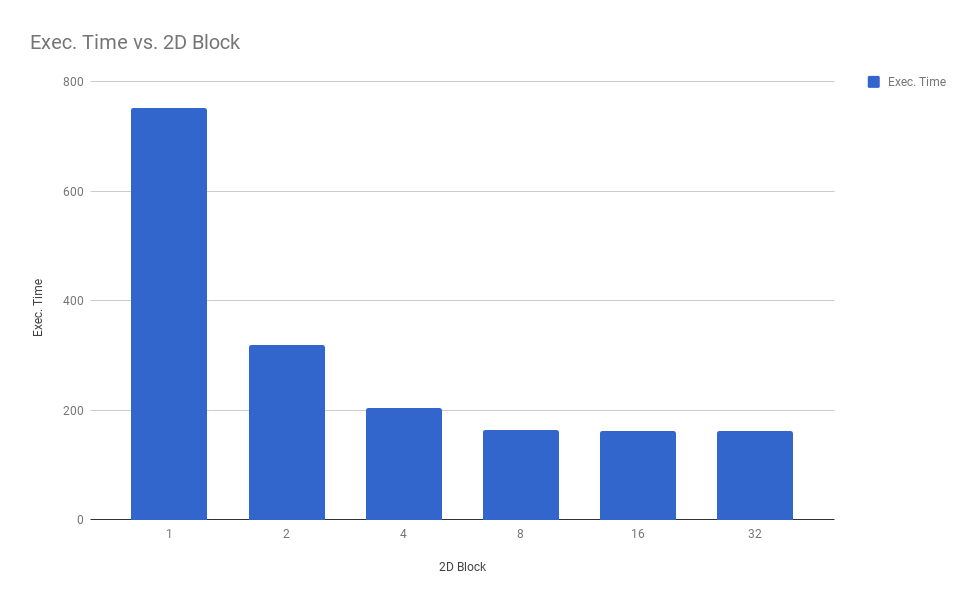
\includegraphics[width=15cm]{chart-gaussian.png}
\centering
\caption{2D Block Size Gaussian Blur Performance Comparison}
\end{figure}
\end{document}